%\documentclass[a4paper, english, 11pt]{article}   
\documentclass[a4paper,12pt,twoside]{article}
\usepackage[T1]{fontenc} 			                  % N�dvendig for fonter
\usepackage[latin1]{inputenc}                   % N�dvendig for ���
\usepackage[english]{babel}						            % Bruk norsk orddeling
\usepackage{graphicx}					                  % For � kunne inkludere grafikk
\usepackage{amsmath, amsfonts, amssymb}         % Pakker for � skrive matte
\usepackage[amssymb]{SIunits}                   % For � bruke \unit til SI-enheter
\usepackage{float}                              % For � bruke H som posisjon
\usepackage[bookmarks]{hyperref}                % For linker til kapitler
\usepackage{url}                                % For � bruke \url
\usepackage{array}                              % For � bruke m{1cm} p� tabell (midtstilt)
\usepackage{changepage}													% Allows for temporary adjustment of side margins
\usepackage{longtable}													% Tables across multiple pages


% Tegninger, som b�ndgap
\usepackage{tikz,tkz-tab}                       % Pakke til � tegne med i latex
\usetikzlibrary{decorations.pathmorphing}       % For � lage foton streker
\usetikzlibrary{decorations.pathreplacing}      % For � bruke kr�llparantes (brace)
\usetikzlibrary{shapes,arrows}                  % For � kunne tegne piler i tikz
\usepackage{xcolor}                             % Farger
\usepackage{rotating}                           % Rotere p� stash
\usepackage{subfigure}                          % Sette figurer ved siden av hverandre
\usepackage{epstopdf}                           % For at .eps figurer skal funke
\DeclareGraphicsExtensions{.pdf,.jpg,.png,.eps} % For � slippe � skrive extensions
\graphicspath{{./images/}}                      % For � slippe � skrive path til bilder

% Info om rapporten
\author{Jon Skarpeteig}
\title{Kryogen mikro-fotoluminiscense p� silisium solcellemateriale}
\date{\today}


\begin{document}

% Tittleside
%\begin{titlepage}
 \thispagestyle{empty}

% \maketitle
 
 \centering
 
 
\includegraphics[width=5cm]{NTNU_engelsk_CMYK}
 
  \vspace{15mm} % Vertikalt mellomrom
 
    \Large
  {\bf{\textsl{Master thesis}}} \\
  
  % Tittel
  \vspace{15mm}          % Vertikalt mellomrom
  \huge
  \textbf{Cryogenic micro-photoluminescence of silicon solar cell materials} \\
  \vspace{4mm}
  \large
  \textbf{by} \\
  \vspace{4mm}
 
  % Forfatter
  \large
  \textbf{Jon Skarpeteig} \\
  \vspace{20mm}

  \large
  \today \\
  \vspace{17mm}
  Supervisors: \\ Helge Weman \\ Arne R�yset \\
  \vspace{15mm} 
  \textsl{Norwegian University of Science and Technology} \\
  \textsl{Department of Electronics and Telecommunications} \\
  
\end{titlepage}

\pagenumbering{roman}

% Sammendrag
%\begin{abstract}
not ready
\end{abstract}


% Innholdsfortegnelser
\clearpage
%\tableofcontents

\clearpage
%\listoffigures

% Faktisk tekst til rapport
\clearpage
\pagenumbering{arabic}
\setcounter{page}{1}

%\input{introduksjon}
\clearpage
%\input{spektroskopi}
%\input{tap}
%\clearpage
Several investigations have documented that dislocations in silicon give rise to characteristic photoluminescence (PL) spectra below the band edge. First showed in \ref{drozdov76} which labeled them D1 (0.812eV), D2 (0.875eV), D3 (0.934eV) and D4 (1.000eV). The samples where deformed at 850 \degrees by bending, so that dislocation densities was inhomogeneous along the samples. \ref{drozdov76} states that the intensity of theese lines increase when the dislocation-rich parts of the crystal is approached. At the same time the intensity of the intrinsic characteristics decrease. The distance between D1-D4 (62 $\pm$ 3 meV) corresponds to the energy of the optical phonons in silicon \ref{drozdov76}. \ref{drozdov76} reports D1 and D2 are dominant in heavily deformed Si crystals, while D3 and D4 predominate in weakly deformed Si. A similar result was also reported by \ref{lee09} for small angle grain boundaries using cathodoluminescence.

\ref{sauer85} suggest that D1-D4 are due to dislocations which have been fronzen in under low-shear stress. Photoluminescence under uniaxial stress shows that D1/D2 originate in the tetragonal defect with random orientation relative to <100> directions. \ref{sauer85} conclude that D3 and D4 are closely related, whereas the independent D1/D2 centers might be deformation-produced point defects in the strain region of dislocations. New lines D5 and D6 emerge when high-temperature, low-stress deformation is followed by low-temperature, high-strss deformation. \ref{sauer85} propose that line D5 is due to straight dislocations and D6 is due to stacking faults. \ref{sauer85} also suggest that D3/D4 photoluminescence is much more characteristic of the dislocations themselves than the D1/D2 emission lines.


The origin of D1 and D2 is not clear. It has been argued that they originate in electronic transition at the geometrical kinks on dislocations \ref{suezawa83}, point defects \ref{sauer85} and impurities \ref{higgs91} and/or from the reaction products of dislocations \ref{sekiguchi95}. On the other hand, D3 and D4 lines is generally thought to be related to electronic transition within dislocation cores \ref{kveder95}. In addition, it has been suggested that the D3 line most likely is a phonon-assisted replica of D4 \ref{kveder95}.




Both \ref{drozdov76} and \ref{sauer85} studied plastically deformed silicon made by the Czochralski process (Cz-Si). \ref{tarasov00} studied  dislocations in multicrystalline silicon (mc-Si) and found similar lines with the entire set of D-lines shifted with around 10meV, presumably due to a strain field. Using a laser annealing technique \ref{staiger94} to introduce dislocations on a Cz-Si wafer, confirm the band location of D1-D4 from \ref{sauer85} in \ref{tarasov00}. A principal difference between dislocation D'-lines in mc-Si versus D-lines in Cz-Si is a substantial broadening (60-70meV at 77K) of the D1'/D2' lines \ref{tarasov00}.


\begin{table}[H]
\centering
\begin{tabular}{|c|c|c|c|c|}
\hline
Cz-Si \ref{drozdov76} & D1 & D2 & D3 & D4 \\
	& 0.812eV & 0.875eV & 0.934eV & 1.000eV \\
\hline
mc-Si \ref{tarasov00} & D1' & D2' & D3' & D4' \\
		& 0.80eV & 0.89eV & 0.95eV & 1.00eV \\
\hline
\end{tabular}
\caption{Energy positions of dislocation D-lines in Cz-Si and D' bands in mc-Si}
\label{}
\end{table}


\ref{tarasov00} reveal a linear dependence of the band-to-band photoluminescence intensity and minority carrier lifetime across entire multicrystalline-Si wafers. Photoluminescence mapping in \ref{tarasov00} of the 0.78eV (0.8eV) band intensity reveal a linkage to areas of a high dislocation density. This band should also be visible in room temperature \ref{tarasov00}.

\ref{tarasov01} later found that if the contamination level is too low, or too high (dislocation decorated by metal silicate precipitates) the defect photoluminescence band vanished in room temperature. However, a relatively low contamination level of dislocations, in the order of 10 impurity atoms per micron of the dislocation length produces distinguishable defect band luminescence \ref{tarasov01}. 

Dislocation related lines (D-lines) has been observed in low temperature photoluminiscence spectra from the regions which included the intragrain defects \ref{sugimoto06}. They also conclude that grain boundaries are not active recombination centers. \ref{sugimoto06} also show a TO-phonon replica of the boron bound exiton at 1.093eV. Intensity of boron bound exiton from the long lifetime regions was higher than that from the short lifetime regions. D-lines reported by \ref{sauer85} are in a short lifetime region. For a long lifetime region, \ref{sugimoto06} observe a peak at 1.00eV which is not the D4 line, but the zonecenter optical phonon sideband of the two-hole transition in the boron bound exiton \ref{dean67}. There have been no reports on the D-line spectrum missing only the D1 line \ref{sugimoto06}.


\ref{sugimoto07} study origins of the defects by low temperature photoluminescence spectroscopy, electron backscatter diffraction pattern measurement and the etch-pit observation, and conclude that defects are metal contaminated dislocation clusters which originated from small angle grain boundaries.






\subsection{Impurities}

Investigation in \ref{higgs92} show that transition-metal contamination plays an important role in the production of D-band luminescence from silicon samples containing either epitaxial stacking faults or oxidation-induced stacking faults. However, \ref{sekiguchi95} later concluded that metallic impurities don't seem to be related to D1 and D2 luminescence.

Room temperature mapping of the 0.77eV band is attributed to oxygen precipitates in in thermally treated silicon made by the Czochralski process (Cz-Si) \ref{tajima95}. This band peak shifts parallel to the bandgap with temperature. The increase of this band on the dislocation lines is due to the preferential precipitation of oxygen \ref{tajima95}.




\ref{inoue07} state that the deep-level emission from multicrystalline silicon with an intensity maximum at 0.78eV at room temperature is diffrent from that of the D1 line at low temperature. Furthermore, \ref{inoue07} suggest that the 0.78eV emission is associated with oxygen precipitation, and that the intra-grain defects are dislocation clusters decorated with oxygen impurities in addition to heavy-metal impurities.

\clearpage
		\section{Abbrevations}
		
		\begin{table}[H]
\centering
\begin{tabular}{|c|c|}
\hline

		\textbf{Abbrevation} & \textbf{Description} \\ \hline
		B$_{TO}$ & TO phonon replica of the Boron bound exiton \cite{sugimoto07} \\ \hline
		BE & Bound exciton \\ \hline
		D$_a$ & Broad background emission \cite{tajima95} \\ \hline
		D$_b$ & Oxygen impurity band \cite{tajima95} \\ \hline
		CZ-Si & Czochralski processed Silicon \\ \hline
		D1	& Dislocation related line 1 \cite{drozdov76} \\ \hline
		D1' & Dislocation related line 1 for mc-Si \cite{tarasov00} \\ \hline
		D2	& Dislocation related line 2 \cite{drozdov76} \\ \hline
		D2' & Dislocation related line 2 for mc-Si \cite{tarasov00} \\ \hline
		D3	& Dislocation related line 3 \cite{drozdov76} \\ \hline
		D3' & Dislocation related line 3 for mc-Si \cite{tarasov00} \\ \hline
		D4	& Dislocation related line 4 \cite{drozdov76} \\ \hline
		D4' & Dislocation related line 4 for mc-Si \cite{tarasov00} \\ \hline
		EBIC & Electron beam induced current \cite{arguirov03} \\ \hline
		EBSP & Electron Backscatter Diffraction Pattern \cite{sugimoto07} \\ \hline
		EHD & Electron Hole Droplet	\\ \hline
		FE & Free exciton \\ \hline
		FZ-Si & Float-zone silicon \\ \hline
		EFG & Edge-define Film-fed Growth \\ \hline
		mc-Si & Multicrystalline silicon \\ \hline
		R1BB & One phonon replica of band edge emission \cite{arguirov03} \\ \hline
		R2BB & Two phonon replica of band edge emission \cite{arguirov03} \\ \hline
		SA GB & Small Angle Grain Boundary \\ \hline
		ZPL & Zero Phonon Line \cite{calao88} \\ \hline

		\end{tabular}
\caption{Abbreviations}
\label{abbreviations}
\end{table}
		
		

%exiton

Free and bound exiton

boron bound exiton

electon hole droplet
%\input{maalemetode}
%\clearpage
%\input{resultater}
%\clearpage
%\input{diskusjon}
%\clearpage
%\input{konklusjon}
%\input{test}

% Referanseliste
\clearpage
\bibliographystyle{plain}
\nocite{}
\bibliography{bibliography} % bibliography.bib

% Vedlegg
\clearpage
\appendix

\section{Silicon energy bands}

\addtolength{\hoffset}{-1.5cm}
\begin{small}
\begin{center}
\begin{longtable}{|c|c|c|c|c|}

% Header for first page
\hline 
\multicolumn{1}{|c|}{\textbf{Energy}} & 
\multicolumn{1}{c|}{\textbf{Name}} & 
\multicolumn{1}{c|}{\textbf{Temp.}} & 
\multicolumn{1}{c|}{\textbf{Impurity / Defect}} & 
\multicolumn{1}{c|}{\textbf{Observed in}} \\ \hline
\endfirsthead


% Header for page 2 3 4 etc.
\multicolumn{5}{c}{{\bfseries \tablename\ \thetable{} -- continued from previous page}} \\
\hline 
\multicolumn{1}{|c|}{\textbf{Energy}} & 
\multicolumn{1}{c|}{\textbf{Name}} & 
\multicolumn{1}{c|}{\textbf{Temp.}} & 
\multicolumn{1}{c|}{\textbf{Impurity / Defect}} & 
\multicolumn{1}{c|}{\textbf{Observed in}} \\ \hline
\endhead

% Table footer on first pages
\hline \multicolumn{5}{|r|}{{Continued on next page}} \\ \hline
\endfoot

% Table footer on last page
\caption{Silicon energy bands}
\label{energy_bands}
\endlastfoot


\hline
0.735eV & ZPL & 22K & Fe contamination & \cite{calao88} \\ \hline
0.745eV & C-N & & Carbon-Nitrogen complex & \cite{davies88} \\ \hline
0.76-0.8eV & Defect & 290K & Dislocation with low contamination & \cite{tarasov00} \cite{tarasov01} \cite{arguirov06} \\ \hline
0.77-0.78eV & D$_b$ & 4.2-295K & Oxygen impurity band & \cite{tajima95} \cite{inoue07} \\ \hline
0.77eV & P line & 12K & C-O complex related & \cite{davies88} \cite{binetti08} \\ \hline
0.780eV & CrB$^{0 \Gamma }$ & 4.2K & CrB$^0$ phonon replica & \cite{conzelmann83} \\ \hline
0.79eV & C-O & 12K & Carbon-Oxygen complex & \cite{davies88} \cite{binetti08} \\ \hline
0.80eV & D1' & 77K & Dislocations \footnotemark[1] & \cite{tarasov00} \cite{tarasov01} \\ \hline
0.812eV & D1 & 4.2K & Dislocation related line \footnotemark[1] & \cite{drozdov76} \cite{sauer85} \cite{arguirov03} \\ \hline
0.8160 & CrB$^2$ & 4.2K & Cr-B excitation of local vibrations & \cite{conzelmann83} \\ \hline
0.8402 & CrB$^1$ & 4.2K & Cr-B excitation of local vibrations & \cite{conzelmann83} \\ \hline
0.8432eV & CrB$^0$ & 4.2K & Cr-B pair no-phonon & \cite{conzelmann83} \\ \hline
0.875eV & C-Ga & & Carbon-Gallium complex & \cite{davies88} \\ \hline
0.875eV & D2 & 4.2K & Dislocation related line \footnotemark[1] & \cite{drozdov76} \cite{sauer85} \cite{arguirov03} \\ \hline
0.89eV & D2' & 77K & Dislocations \footnotemark[1] & \cite{tarasov00} \cite{tarasov01} \\ \hline
0.8-0.9eV & D$_{a1}$ & 11K & Broad background emission under D1/D2 & \cite{tajima95} \\ \hline
0.91eV & H-line & 12K & C-O complex related & \cite{davies88} \cite{binetti08} \\ \hline
0.93eV & H-line & 12K & C-O complex related & \cite{davies88} \cite{binetti08} \\ \hline
0.934eV & D3 & 4.2K & Dislocations \footnotemark[2] & \cite{drozdov76} \cite{sauer85} \cite{arguirov03} \\ \hline
0.95eV & D3' & 77K & Dislocations \footnotemark[2] & \cite{tarasov00} \cite{tarasov01} \\ \hline
0.953eV & D5 & 4.2K & Straight dislocations & \cite{sauer85} \cite{weronek91} \\ \hline
0.968eV & I$^{TO+20^\Gamma}$ & 26K & TO + 2 Zone center phonon & \cite{dean67} \\ \hline
0.969eV & C-C & & Carbon-Carbon complex & \cite{davies88} \\ \hline
0.98eV & R2BB & 80K & Two phonon replica of band edge emission & \cite{arguirov03} \\ \hline
0.9-1.0eV & D$_{a2}$ & 11K & Broad background emission under D3/D4 & \cite{tajima95} \\ \hline
1.000eV & D4 & 4.2K & Dislocations \footnotemark[2] & \cite{drozdov76} \cite{sauer85} \cite{arguirov03} \\ \hline
1.00eV & D4' & 77K & Dislocations \footnotemark[2] & \cite{tarasov00} \cite{tarasov01} \\ \hline
1.0089eV & FeB$^0$(TO) & 6K & Fe-B pair phonon replica & \cite{mohring83} \\ \hline
1.0126eV & D6 & 4.2K & Stacking faults & \cite{sauer85} \cite{weronek91} \\ \hline
1.013eV & I$^{TO+0^\Gamma+IV^a}$ & 26K & $TO+0^ \Gamma +IV^a$ phonon & \cite{dean67} \\ \hline
1.014eV & Cu$_0$ & 4.2K & Copper doping & \cite{weber82} \cite{weronek91} \\ \hline
1.018eV & W/I1 & & Radiation damage & \cite{davies88} \\ \hline
1.0315eV & I$^{TO+0^ \Gamma}$ & 26K & TO + Zone center phonon & \cite{dean67} \\ \hline
1.04eV & R1BB & 80K & One phonon replica of band edge emission & \cite{arguirov03} \\ \hline
1.045eV & Q & & 4-Li atom complex & \cite{davies88} \\ \hline
1.0504eV & FeB$^{2}$ & 6K & Fe-B pair contamination & \cite{mohring83} \\ \hline
1.051eV & I$^{TO+IV^b}$ & 26K & Inter valley phonon replica & \cite{dean67} \\ \hline
1.0595eV & FeB$^{1}$ & 6K & Fe-B pair contamination & \cite{mohring83} \\ \hline
1.0692eV & FeB$^{0}$ & 6K & Fe-B pair no phonon & \cite{mohring83} \\ \hline
1.074eV & I$^{TO+IV^a}$ & 26K & Inter valley phonon replica & \cite{dean67} \\ \hline
1.078 & EHD & 4.2K & Electron Hole Droplet dislocation-area & \cite{drozdov03} \\ \hline
1.082eV & EHD$_{TO}$ & 4.2K & Electron Hole Droplet dislocation-free & \cite{hammond75} \cite{drozdov03} \cite{satoshi04} \\ \hline
1.0835eV & In$^{TO}$ & 30K & Indium doping TO & \cite{dean67} \\ \hline
1.0888eV & Bi$^{TO}$ & 15K & Bismuth doping TO & \cite{dean67} \\ \hline
1.0902eV & Al$^{TO}$ & 30K & Aluminum doping TO & \cite{dean67} \\ \hline
1.0907eV & As$^{TO}$ & 15K & Arsenic doping TO & \cite{dean67} \\ \hline
1.0907eV & Ga$^{TO}$ & 15K & Gallium doping TO & \cite{dean67} \\ \hline
1.0916eV & P$^{TO}$ & 15K & Phosphorus doping TO & \cite{dean67} \\ \hline
1.092eV & BE1 & 4.2K & Bound exciton & \cite{drozdov76} \\ \hline
1.0921eV & Sb$^{TO}$ & 15K & Antimony doping TO & \cite{dean67} \\ \hline
1.0970eV & I$^TO$/FE & 26K & Transversal Optical/Free exciton & \cite{dean67} \cite{hammond75} \cite{drozdov03} \\ \hline
1.0924eV & B$^{TO}$ & 15K & Boron doping TO & \cite{dean67} \\ \hline
1.093eV & B$_{TO}$ & 4.2K & TO phonon replica of Boron bound exciton & \cite{sugimoto07} \cite{inoue07} \\ \hline
1.1365eV & I$^TA$/LO/FE & 26K & Transversal Acoustic/Longitudinal/FE & \cite{hammond75} \cite{dean67} \\ \hline
1.1545eV & I$^0$ & 26K & No phonon & \cite{dean67} \\ \hline

%1.25eV? EHD$^{TO}$ \cite{sauer85}
%1.26eV? Fe$^{TO}$ \cite{sauer85}
%BE \cite{inoue07}

\end{longtable}
\end{center}
\end{small}

\footnotetext[1]{D1 and D2:	It has been argued that they originate in electronic transition at the geometrical kinks on dislocations \cite{suezawa83}, point defects \cite{sauer85} and impurities \cite{higgs91} and/or from the reaction products of dislocations \cite{sekiguchi95}.}
	
\footnotetext[2]{D3 and D4 lines is generally thought to be related to electronic transition within dislocation cores \cite{kveder95}. In addition, it has been suggested that the D3 line most likely is a phonon-assisted replica of D4 \cite{kveder95}.
}


%%%%%%%%%%%%%%%%%%%%%%%%%%%%%%%
\clearpage
\section{Sample types and procedures}

\begin{figure}[H]
\centering
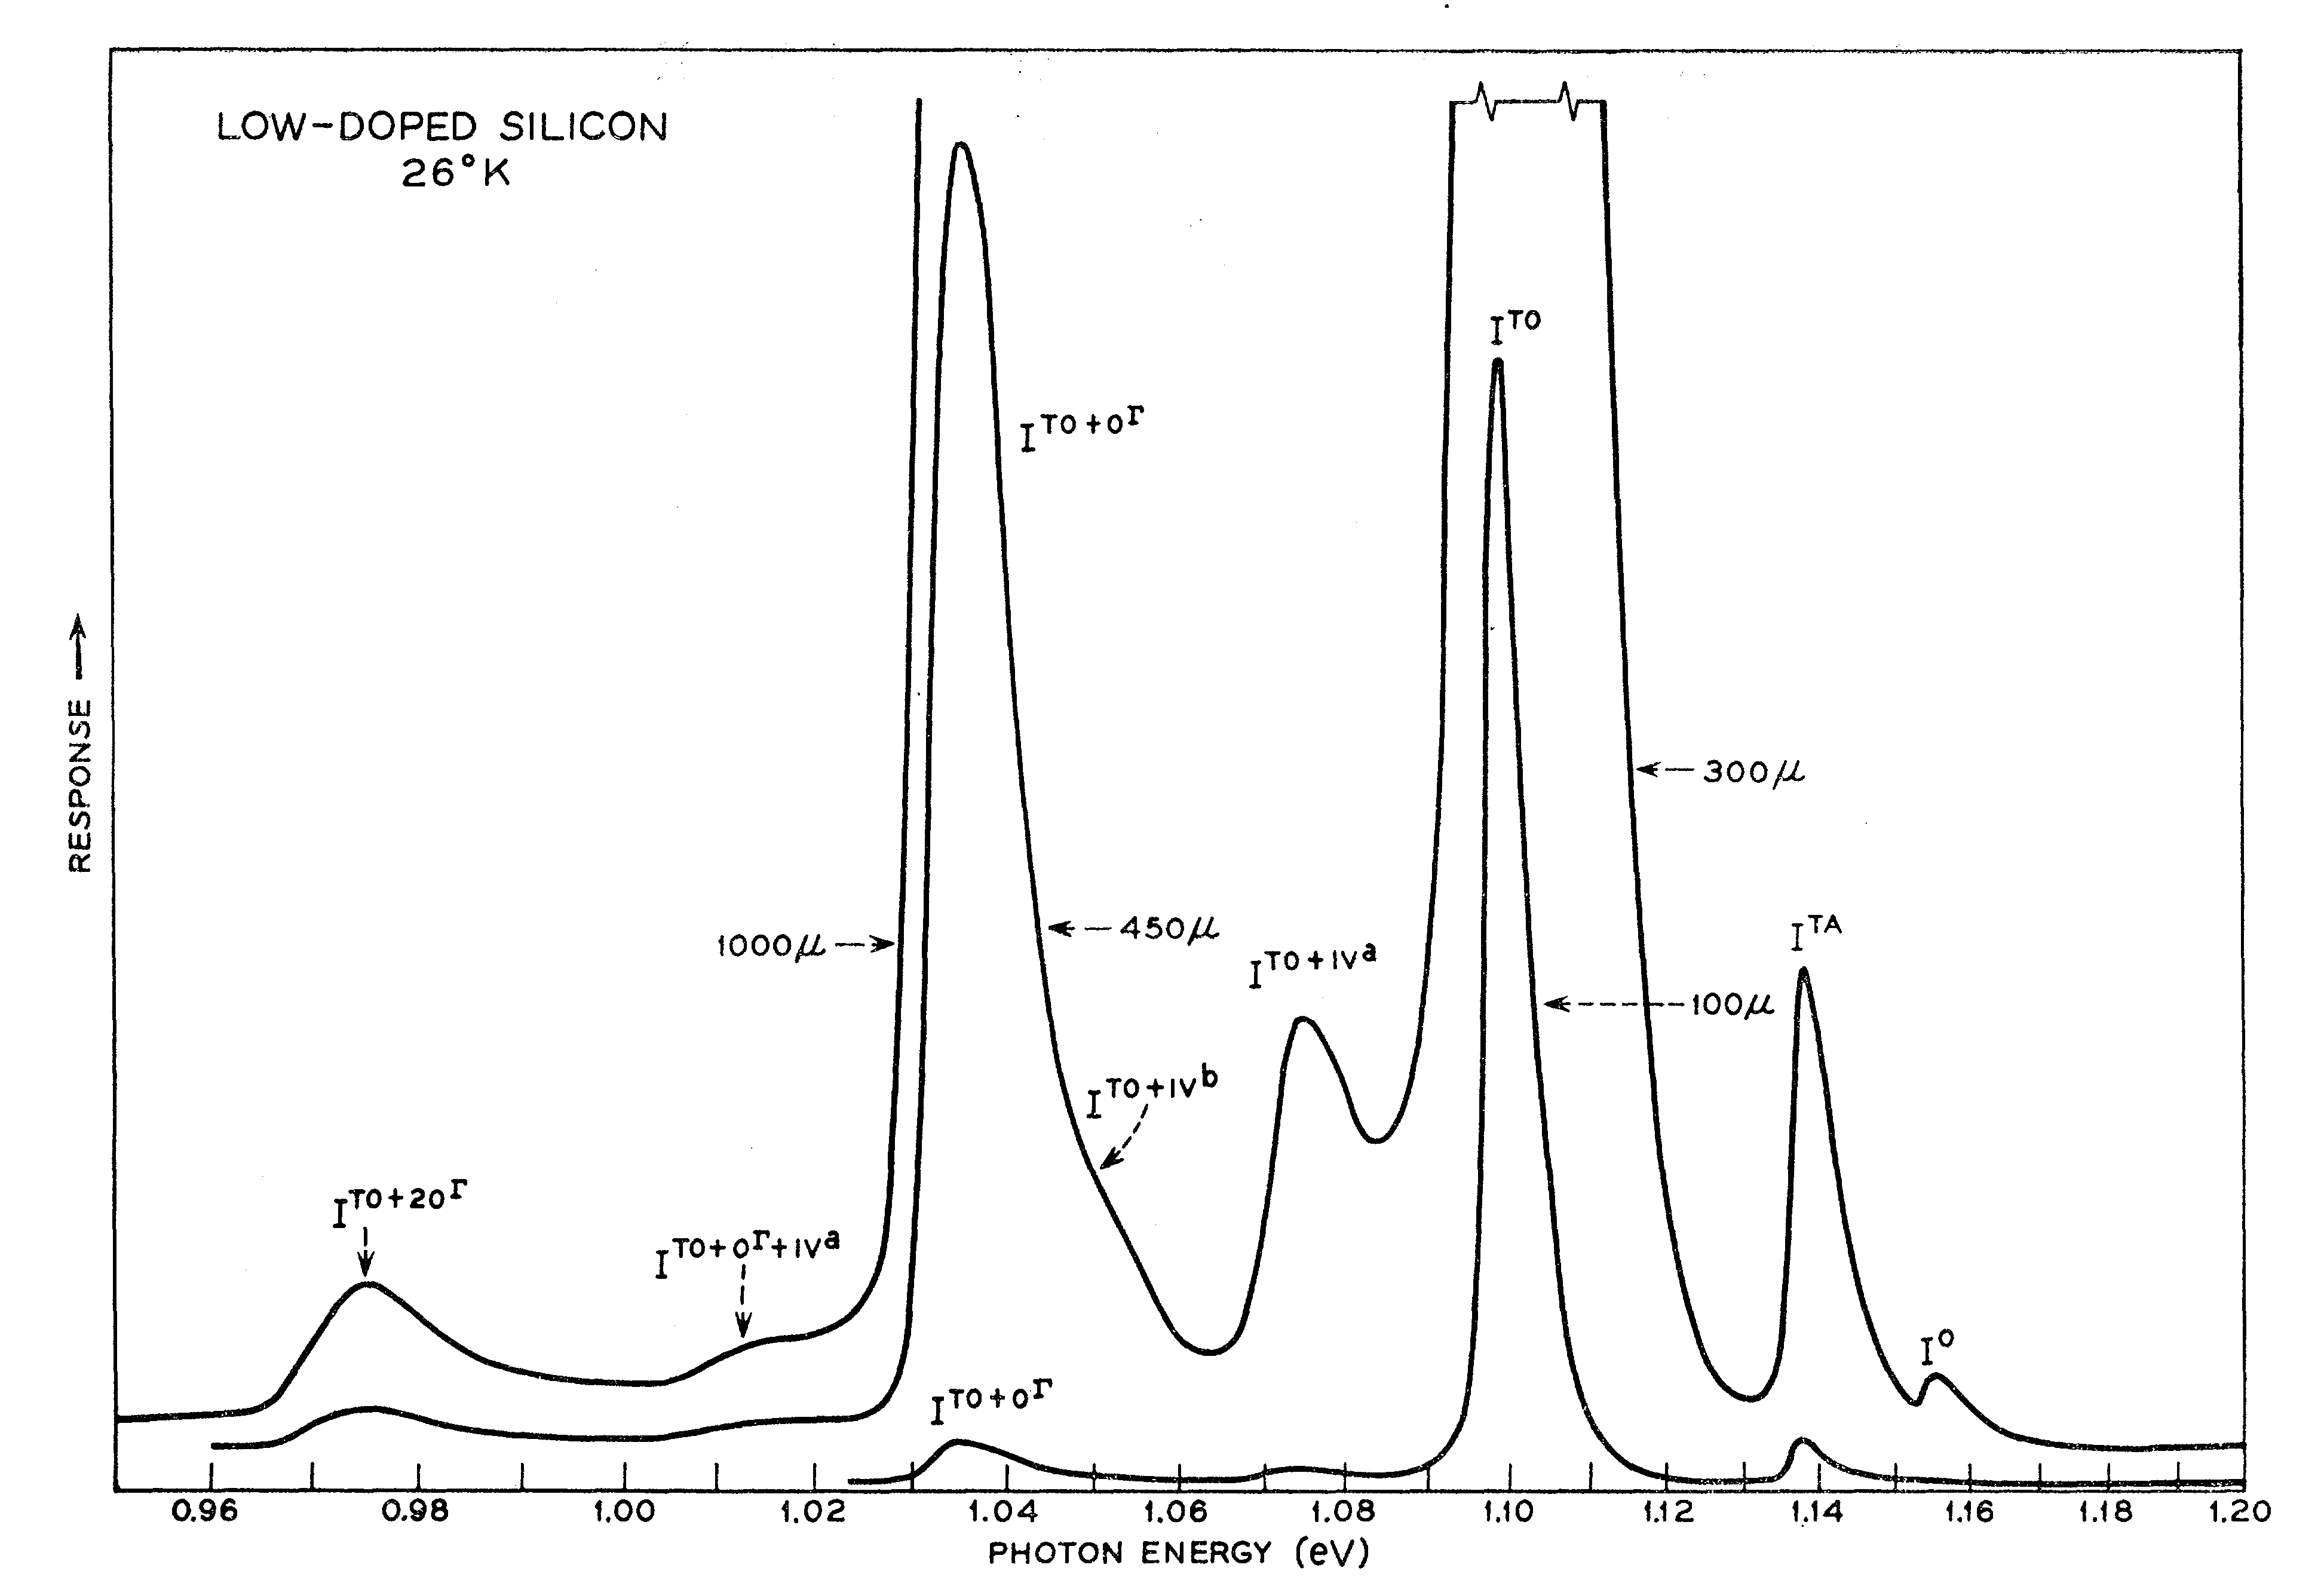
\includegraphics[width=15cm]{n-type_Si_spectra_dean67}
\caption{Low doped ($2\cdot10^{14}cm^{-3}$ P atoms) n-type Si PL specter from \cite{dean67}}%
\label{fig:SiPL}%
\end{figure}

\begin{figure}
\centering
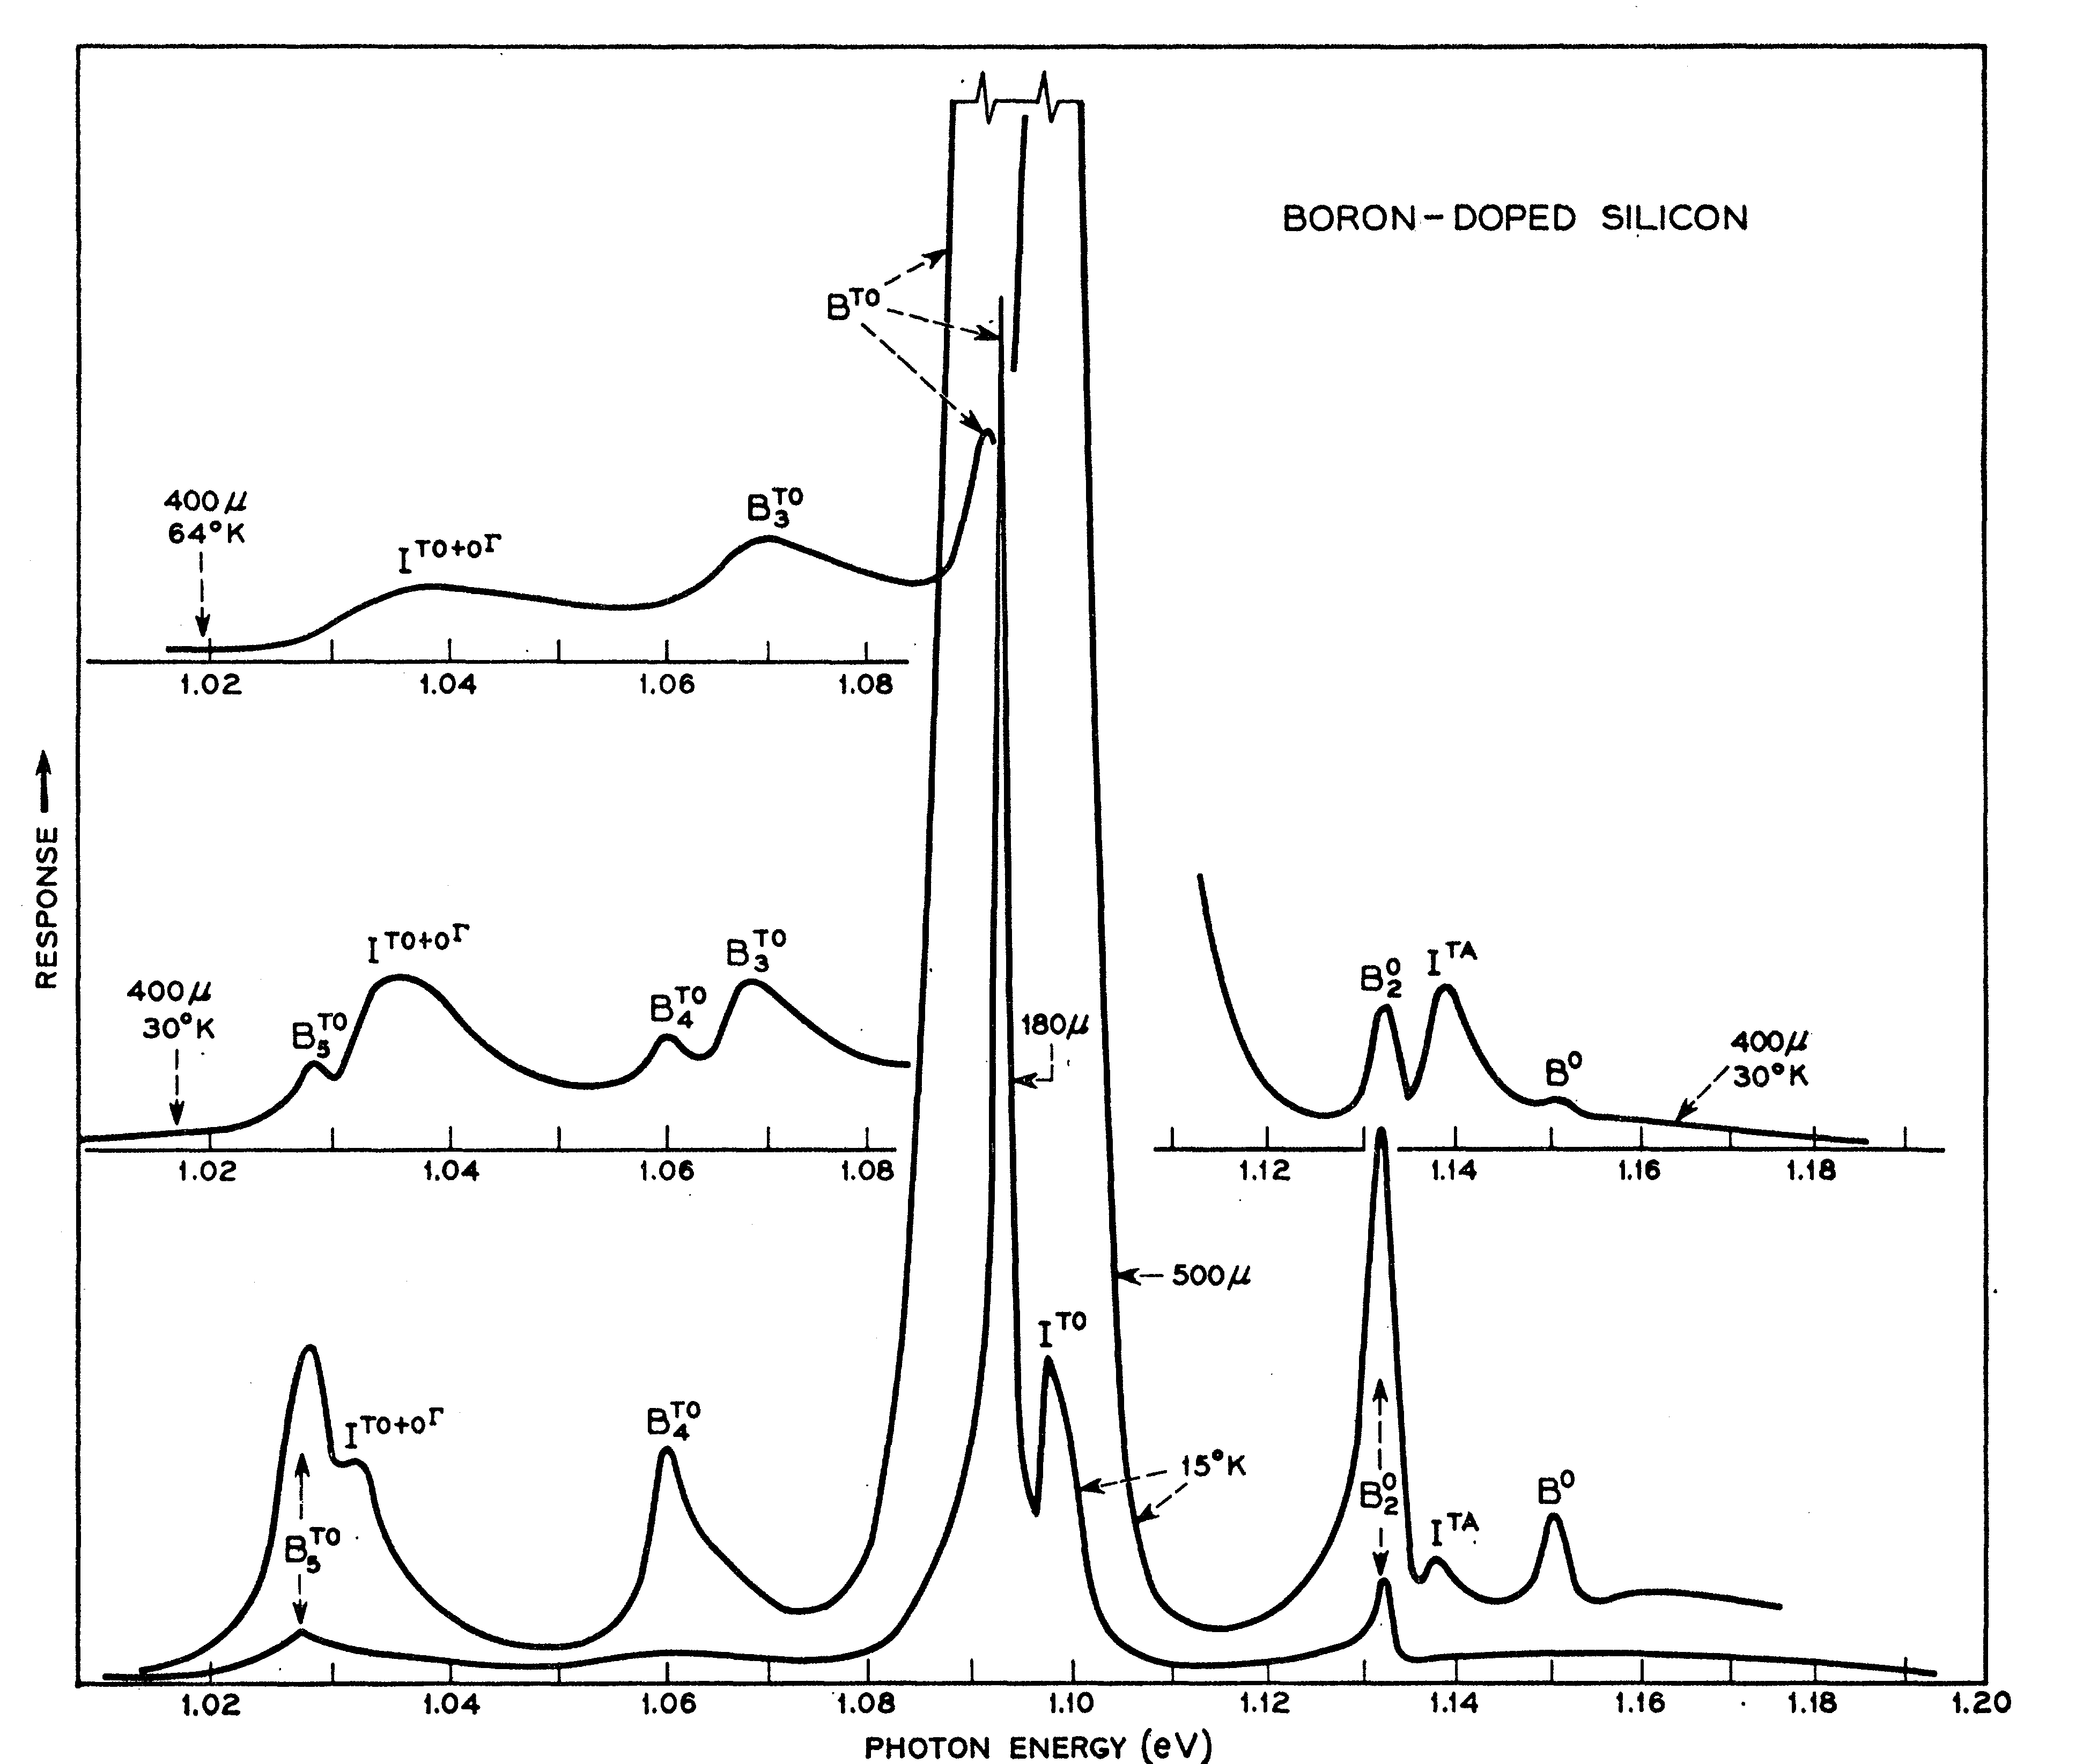
\includegraphics[width=15cm]{boron_Si_spectra_dean67}
\caption{Boron doped ($6\cdot10^{16}cm^{-3}$) Si PL specter from \cite{dean67}}%
\label{fig:boronSiPL}%
\end{figure}


\begin{figure}
\centering
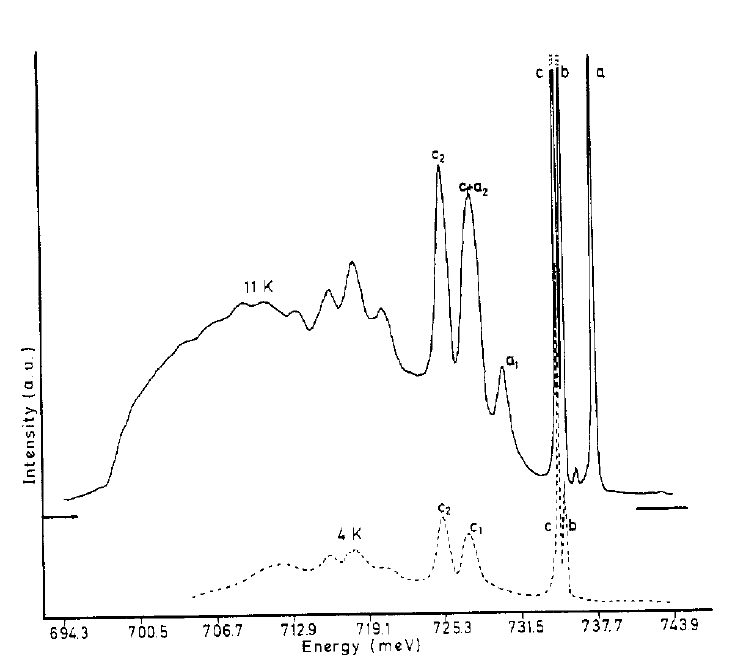
\includegraphics[width=15cm]{iron_diffused_Si_spectra}
\caption{Iron diffused Si sample at two different temperatures from \cite{calao88}}%
\label{fig:FeSiPL}%
\end{figure}


\begin{figure}
\centering
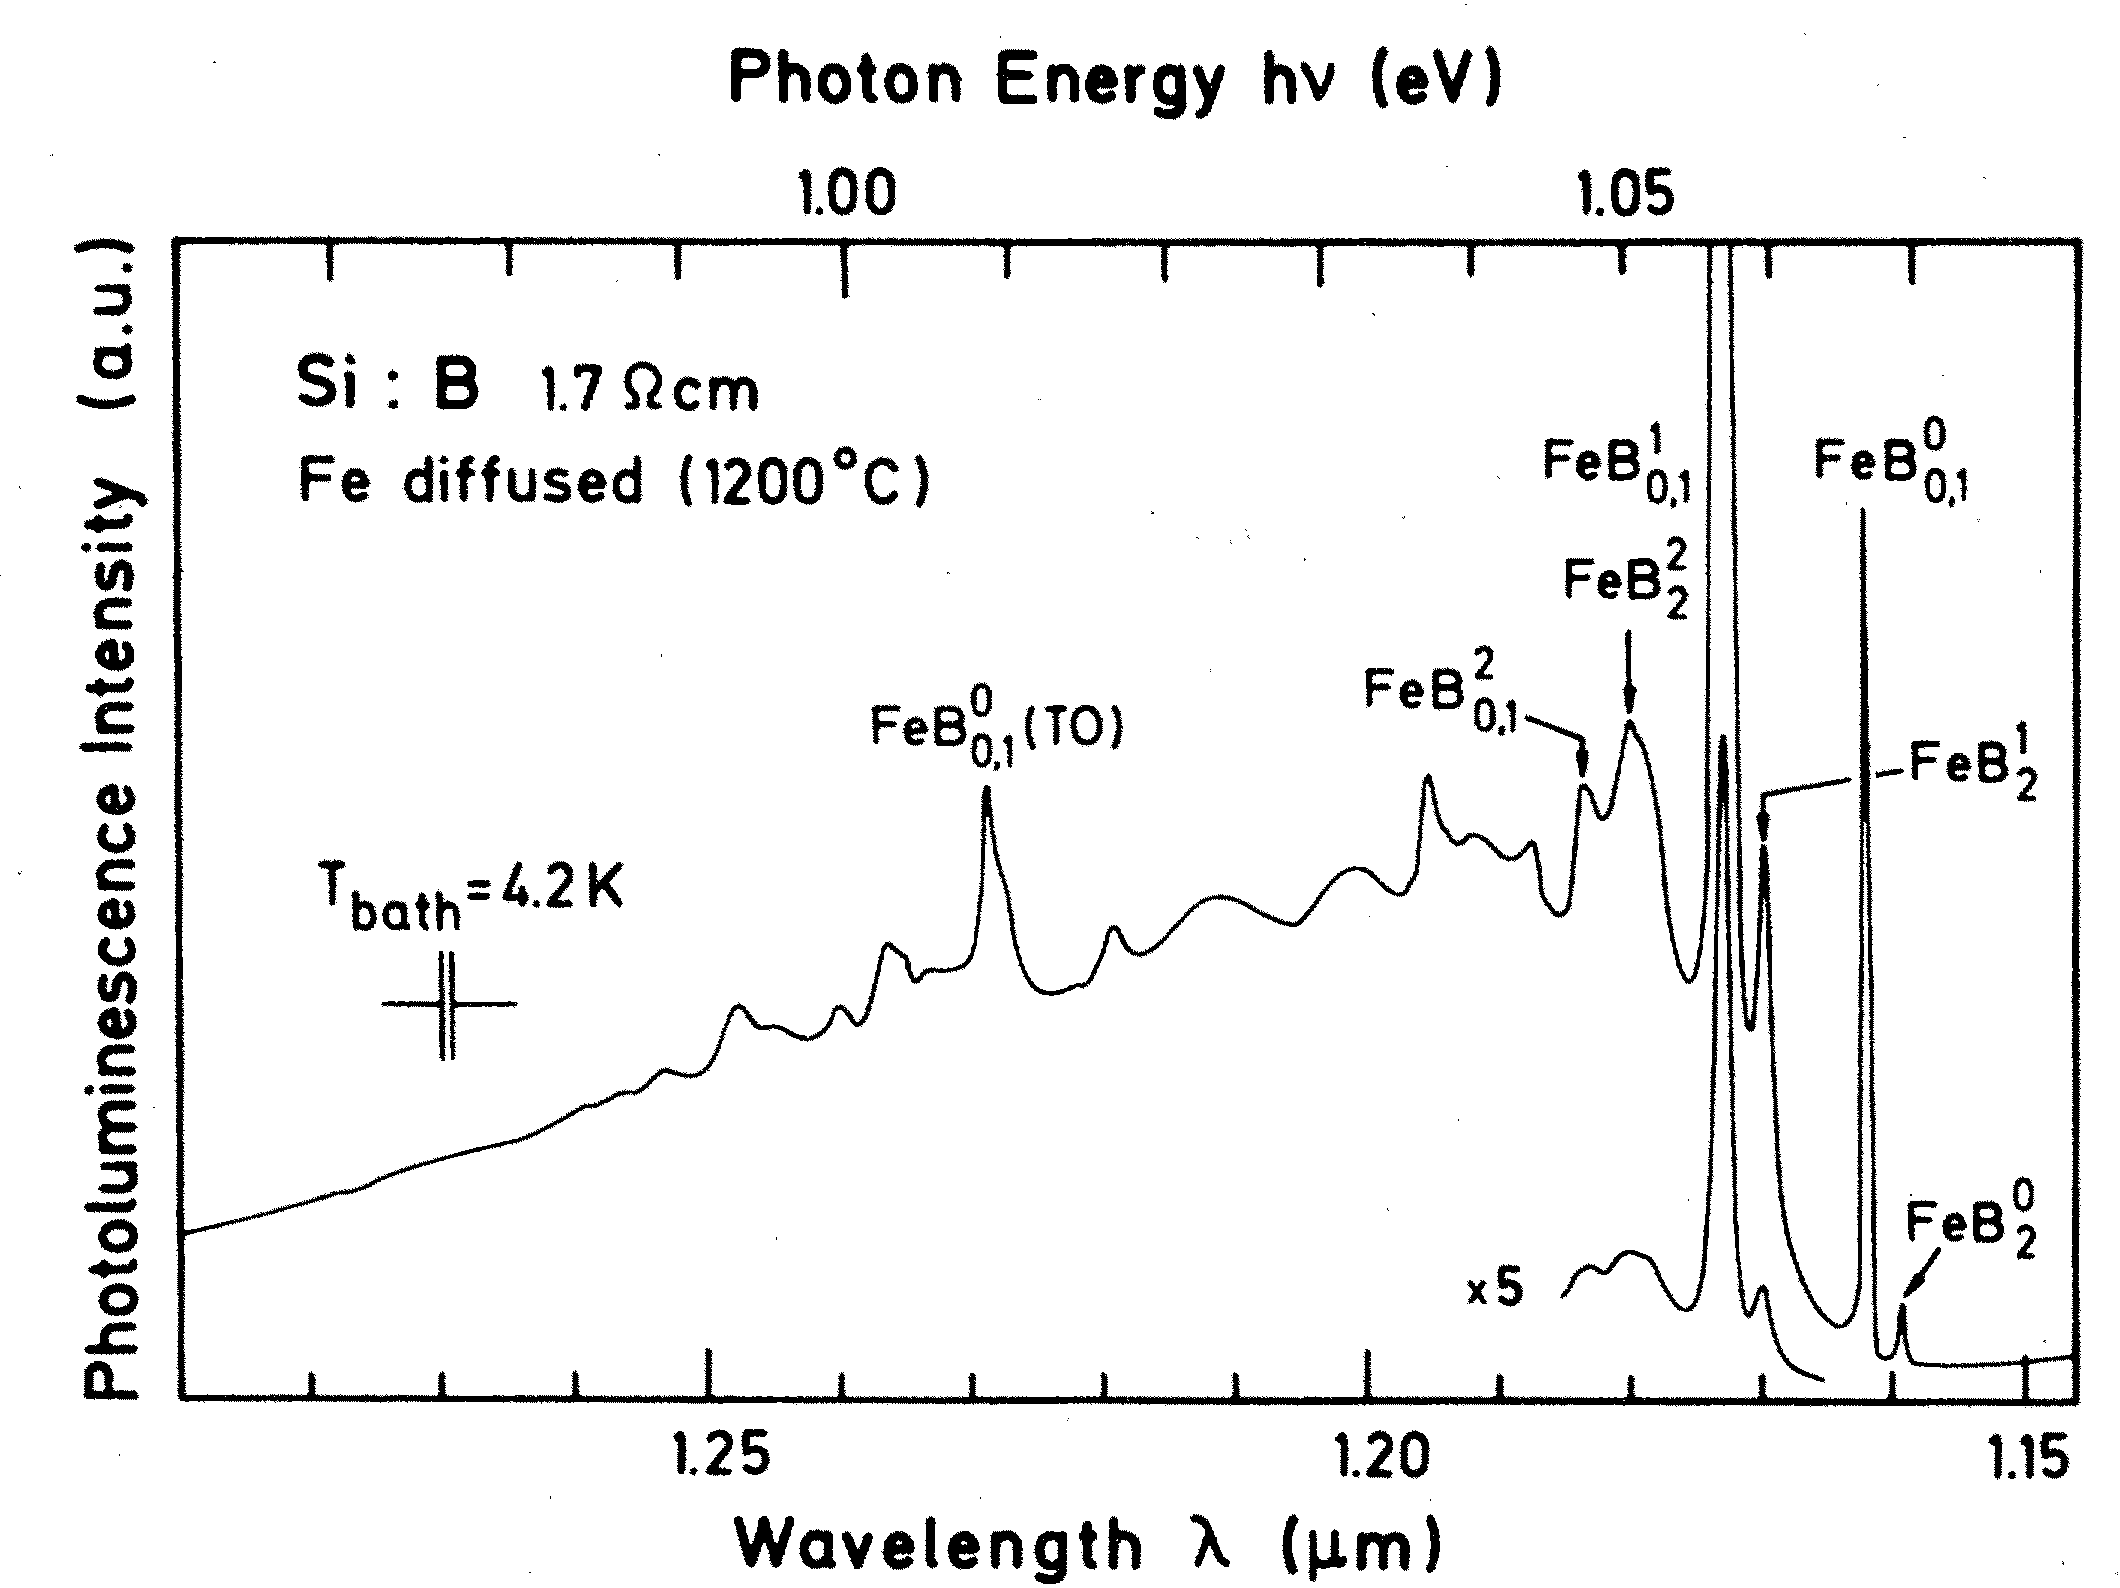
\includegraphics[width=15cm]{iron_diffused_boron_doped_Si_spectra}
\caption{Iron diffused boron doped Si sample from \cite{mohring83}}%
\label{fig:FeBSiPL}%
\end{figure}

\begin{figure}
\centering
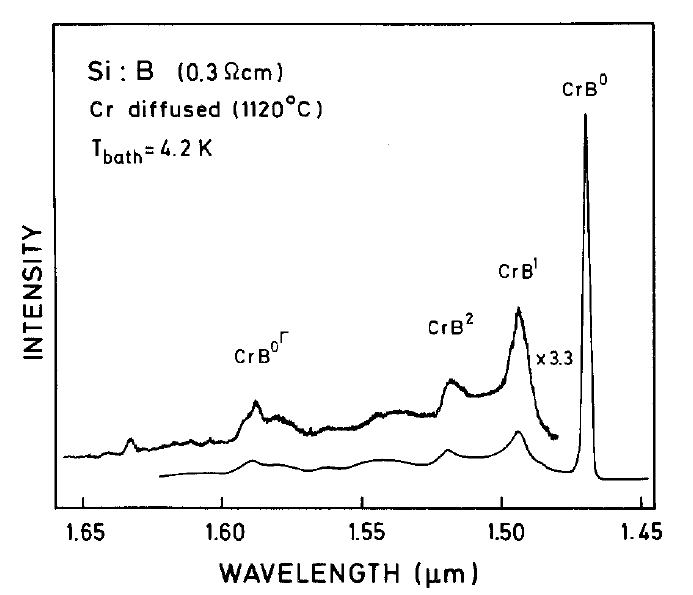
\includegraphics[width=15cm]{CrB_Si_spectra}
\caption{Chromium diffused Boron doped Si sample from \cite{conzelmann83}}%
\label{fig:CrBSiPL}%
\end{figure}


\addtolength{\hoffset}{+1.5cm}
\begin{center}
\begin{sidewaystable}%
\small \begin{tabular}{|c|c|m{3cm}|m{4cm}|m{4cm}|m{2cm}|}

% Header for first page
%\hline 
%\multicolumn{1}{|c|}{\textbf{Ref.}} & 
%\multicolumn{1}{c|}{\textbf{Sample type}} & 
%\multicolumn{1}{c|}{\textbf{Excitation process}} & 
%\multicolumn{1}{c|}{\textbf{Area}} & 
%\multicolumn{1}{c|}{\textbf{Surface process}} & 
%\multicolumn{1}{c|}{\textbf{Doping}} \\ \hline
%\endfirsthead

% Header for page 2 3 4 etc.
%\multicolumn{6}{c}{{\bfseries \tablename\ \thetable{} -- continued from previous page}} \\
%\hline 
%\multicolumn{1}{|c|}{\textbf{Ref.}} & 
%\multicolumn{1}{c|}{\textbf{Sample type}} & 
%\multicolumn{1}{c|}{\textbf{Excitation process}} & 
%\multicolumn{1}{c|}{\textbf{Area}} & 
%\multicolumn{1}{c|}{\textbf{Processing}} & 
%\multicolumn{1}{c|}{\textbf{Doping}} \\ \hline\endhead

% Table footer on first pages
%\hline \multicolumn{6}{|r|}{{Continued on next page}} \\ \hline
%\endfoot

% Table footer on last page
%\endlastfoot
\hline
\textbf{Ref.} & \textbf{Sample type} & \textbf{Excitation process} & \textbf{Area} & \textbf{Processing} & \textbf{Doping} \\ \hline

\cite{sugimoto07} & mc-Si & 532nm Nd:YVO$_4$ & $0.1mW/10$ $�$m diameter & Sawing damage etched by HNO$_3$/HF & B-doped \\ \hline
\cite{tajima95} & Cz-Si & Kr ion laser 647nm & 10 \micro m &  & Undoped \\ \hline
\cite{drozdov76} & Cz-Si & Xenon lamp & 50mW on 3mm modulated at 9Hz & deformed by bending at 850$^\circ$ C & undoped, weak n and p \\ \hline
\cite{tarasov00} & mc-Si & 800nm AlGaAs laser & Pulsed 300mW / 3mm &  & Block-casting technique for Baysix \\ \hline
\cite{tarasov01} & mc-Si & 800nm AlGaAs at 140mW & & Produced by EFG & \\ \hline
\cite{arguirov03} & mc-Si and FZ-Si & Ar ion 514nm at 300mW & 100\micro m & Produced by EFG & boron doped $10^15cm^-1$ \\ \hline
\cite{sauer85} & FZ-Si & Kr-ion 647nm, Ar-ion 415nm and Nd-YAG 1064nm &  & Deformed a 650$^\circ$ C and 850$^\circ$ C & residual $10^{12}$cm$^{-3}$ boron \\ \hline
\cite{inoue07} & mc-Si & Nd:YVO 532nm & 6mW, 10$�$m diameter & Slicing damage etched off by HNO$_3$/HF & boron doped \\ \hline
\cite{conzelmann83} & FZ-Si and CZ-Si & & 50mW laser & Etched with HNO$_3$/HF. Chromium diffused & boron doped \\ \hline
\cite{mohring83} & FZ-Si & Ar$+$ 514nm & 500mW & Fe diffused & boron doped \\ \hline
\cite{calao88} & FZ-Si & Argon laser & & Fe diffusion & undoped \\ \hline
\cite{weber82} & & Ar$^+$ 514nm at 1.5W & & & Cu doped \\ \hline
\cite{weronek91} & FZ-Si & Ar$^+$ 514nm & & Heated above a Bunsen burner & Doped with Cu and/or Fe \\ \hline
\cite{binetti08} & mc-Si & & 6W/cm$^2$ & Polished by HNO$_3$/HF & Undoped \\ \hline
\cite{dean67} & CZ-Si & 200W mercury arc ~2.5eV & & & Undoped and doped \\ \hline
\cite{drozdov03} &  & Ar$^+$ or Kr$^+$ laser 0.6W & 0.8mm diameter & Dislocations by bending at ~700$^ \circ$C & phosphorus doped \\ \hline

\end{tabular}

\caption{Sample types and procedures}
\label{tab:sample_types}

\end{sidewaystable}
\end{center}



%\input{vedlegg_transmisjon}

\end{document}